\documentclass[pdftex,12pt,a4paper]{report}

\usepackage[utf8]{inputenc}
\usepackage[T1]{fontenc}
\usepackage[francais]{babel}
\usepackage{setspace}
\usepackage[top=2.5cm,bottom=2.5cm,right=3cm,left=3cm]{geometry}
\usepackage{parskip}

\usepackage{hyperref}
\usepackage{color}

\usepackage{calc}
\usepackage{pseudocode}

\usepackage[pdftex]{graphicx}
\usepackage{float}
\usepackage{caption}
\usepackage{fancybox}

\usepackage{caption}
\captionsetup{figurewithin=none}  
\captionsetup{tablewithin=none}

\AddThinSpaceBeforeFootnotes

\FrenchFootnotes

\newcommand{\HRule}{\rule{\linewidth}{1mm}}

\setlength{\parskip}{1mm}

\begin{document}

\begin{titlepage}
  \begin{sffamily}
  \begin{center}

    % Upper part of the page. The '~' is needed because \\
    % only works if a paragraph has started.
    
\includegraphics[scale=0.6]{./img/univ-lille1.png}~\\[1.5cm]
    
    \textsc{\Large Master INFORMATIQUE}\\[0.5cm]
    
    \textsc{\Large Mention INFORMATIQUE}\\[2cm]

    \textsc{\LARGE Rapport de ProJet Encadré}\\[2cm]

    % Title
    \HRule \\[0.4cm]
    { \huge \bfseries Analyse de Comportements avec Twitter\\[0.4cm] }

   \vfill

    % Author and supervisor
    \begin{minipage}{0.4\textwidth}
      \begin{flushleft} \large
        Antonin \textsc{Carette}\\
        Alexandre \textsc{Verkyndt}\\
      \end{flushleft}
    \end{minipage}
    
    \vfill

    % Bottom of the page
    {\large Promo 2014/2015}

  \end{center}
  \end{sffamily}
\end{titlepage}

\begin{spacing}{1.2}

\tableofcontents

\chapter*{Introduction}

\addcontentsline{toc}{chapter}{Introduction} 

\section{Problèmatique}

Le but de ce projet était de réaliser une application permettant d'analyser les comportements de tweets contenus dans l'application Twitter (en particulier, l'analyse de sentiments), via l'utilisation de son interface de programmation.\\
L'analyse de comportements sera étudié via différents algorithmes de classification (ou modèle), utilisant ou non une base d'apprentissage : le modèle basique (basé sur des dictionnaires), le modèle KNN et enfin le modèle Bayesien.

\section{Interface de programmation Twitter}

Pour ce projet, nous allons utiliser l'interface de programmation\footnote{Une interface de programmation est aussi appelée "API".} de Twitter.\\
Cette API nous permettra de récupérer les tweets voulus, sur un sujet donné, ainsi que toutes les informations suivantes : l'ID du tweet, l'émetteur, s'il s'agit d'un tweet original ou s'il s'agit d'un \textit{retweet}\footnote{Un \textit{retweet} est un tweet partagé - il n'est alors en aucun cas original.}.\\
Aussi, nous allons utiliser cette interface via la librairie Java \textit{Twitter4J}, dans sa version stable. En effet, cette librairie (à jour en fonction des mises à jour de l'interface de programmation) Java nous permettra d'accéder facilement aux tweets recueillis ainsi qu'aux informations du tweet, via des classes et des méthodes Java programmées.

\chapter{Présentation du logiciel}

\section{Généralités}

Ce programme a été écrit avec Java et Swing, pour la partie Interface Utilisateur.
\\
Suite à l'utilisation de fonctions avancées telles que le \textit{switch} sur une chaîne de caractères, ou le \textit{cast} des JComboBox, ce programme n'est compatible qu'avec une Machine Virtuelle Java de version 7 et plus.

\subsection{Titre et logo}

Notre logiciel se nomme \textit{BehAnTweet}\footnote{La documentation développeur du logiciel est présente dans le répertoire \textit{\textbf{doc}}, à partir de la racine du projet.}. Le nom du logiciel se réfère à une phrase anglaise "Behavior Analysis of a Tweet", littéralement "Analyse de Comportement d'un Tweet", sujet du projet encadré.
\\
Le logo du logiciel est, quant à lui, une référence à \textit{Bahamut}\footnote{Un poisson (ou serpent géant), présent dans la mythologie Arabe.}, sous licence libre.

\subsection{Logiciels de versioning}

Git a été utilisé comme logiciel de versioning principal, dû à sa simplicité d'emploi, à la durée d'utilisation faite de celui-ci depuis plusieurs mois ainsi que grâce à l'application interactive Github\footnote{https://github.com/WebTogz/BehAnTweet}.\\
Svn a lui été utilisé pour transmettre la version principale du logiciel sur les serveurs de l'Université, toutes les 3 semaines, afin de pouvoir visualiser l'avancement du projet régulièrement.

\section{Description de l'architecture de l'application}

Nous avons utilisé le modèle \textbf{MVC} (pour Modèle - Vue - Contrôleur) pour notre projet.\\
Ce modèle, très connu pour le développement logiciel, est destiné à répondre aux besoins des applications interactives, en séparant les problématiques liées aux différents composants au sein de leur architecture respective.\\
Aussi, le gros bénéfice de ce patron est qu'il permet facilement l'évolution de l'application par la suite, via l'ajout de classes dans les packages spécifiques suivants: \textbf{Controler}, \textbf{Model}, \textbf{View}.

\subsection{Packaging}

\subsubsection{Controler}

Le contrôleur prend en charge la gestion des événements de synchronisation pour mettre à jour la vue ou le modèle, et les synchroniser. Il analyse la requête du client et se contentera alors renvoyer la vue correspondant à la demande, en fonction du modèle appelé. Aussi, il est important de savoir que le contrôleur n'effectue aucun traitement, et ne modifie aucunement les données!
\\
Il était ainsi nécessaire d'implémenter le patron \textbf{Observable/Observeur}, afin de pouvoir un Observer (objet qui observe) qu'une modification a été apporté sur un Observable (objet observé par un Observer).

\subsubsection{Model}

Le modèle est le coeur algorithmique de l'application - il gère le traitement des données, la modification des vues mais aussi les interactions avec la base de données.
\\
Le package Model contiendra tous les modèles de l'application - chaque modèle (à part la base Model.java) contiendra sa propre implémentation d'un algorithme de classification (Dictionnaire, KNN, Bayes).

\subsubsection{View}

La vue est le coeur de l'intéraction avec l'application.
\\
Elle détient plusieurs tâches à effectuer:
\begin{itemize}
\item{la première est de présenter les résultats renvoyés par le modèle,}
\item{la seconde est de recevoir l'action de l'utilisateur - via la manipulation de boutons, objets cliquables, etc...}
\end{itemize}
Toutes ces tâches, une fois finalisées, seront renvoyées au Contrôleur de l'application afin de pouvoir être traitées par le modèle.

\section{Interface graphique}

Nous avons pensé avant tout à une utilisation simple du logiciel, reposant sur une seule fenêtre. Cette fenêtre contiendra tous les paramètres pouvant être manipulés par l'utilisateur (le nombre de tweets à recueillir, l'algorithme utilisé et ses spécifications), une barre de recherche concernant un sujet donné, et enfin un grand espace dédié à la liste des tweets recueillis et de leur classification par l'algorithme choisi.

\subsection{Captures d'écran}

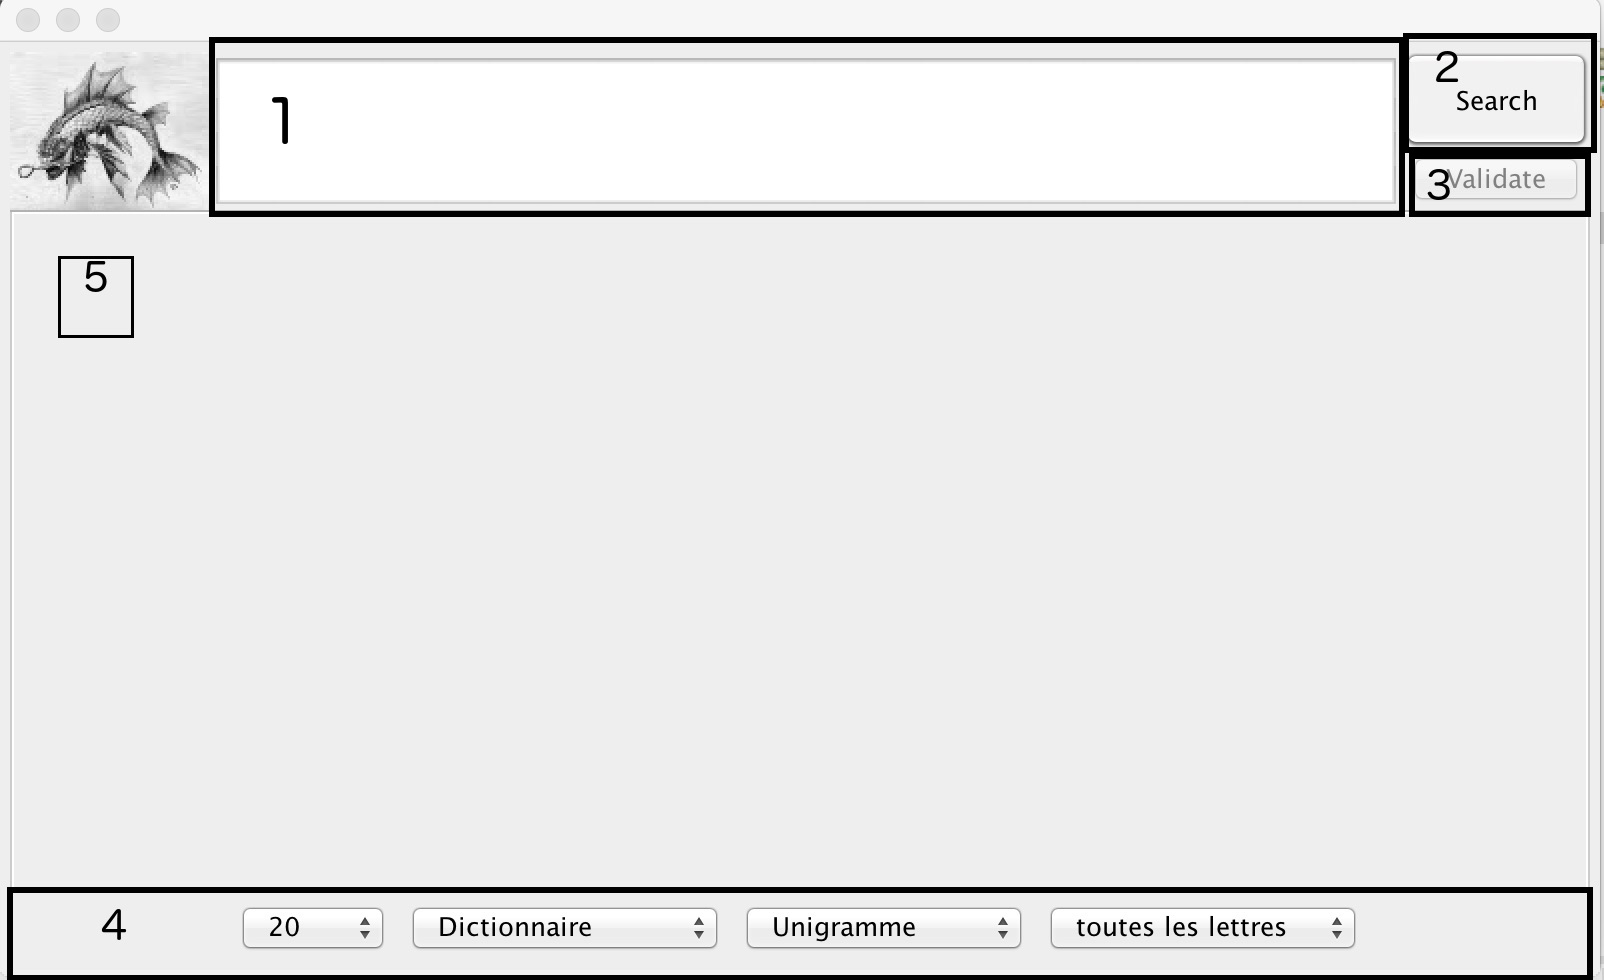
\includegraphics[scale=0.5]{img/BehAnTweet_annotation.jpeg}

Voici l'écran principal de l'application. Il est constitué en 3 grandes parties, pouvant être divisées à leur tour.
\begin{itemize}
\item{\textbf{encart de recherche} : barre de recherche de tweet\textbf{(1)}, bouton de recherche\textbf{(2)}, bouton de validation\textbf{(3)} - permet la validation des tweets recueillis après vérification des comportements,}
\item{\textbf{encart de paramètres} : paramètres ajustables de l'application\textbf{(4)} - permet la modification du nombre de tweets à recueillir, de la méthode de classification à utiliser, ainsi que les paramètres KNN,}
\item{\textbf{encart de visualisation} : visualisation des tweets recueillis\textbf{(5)}.}
\end{itemize}

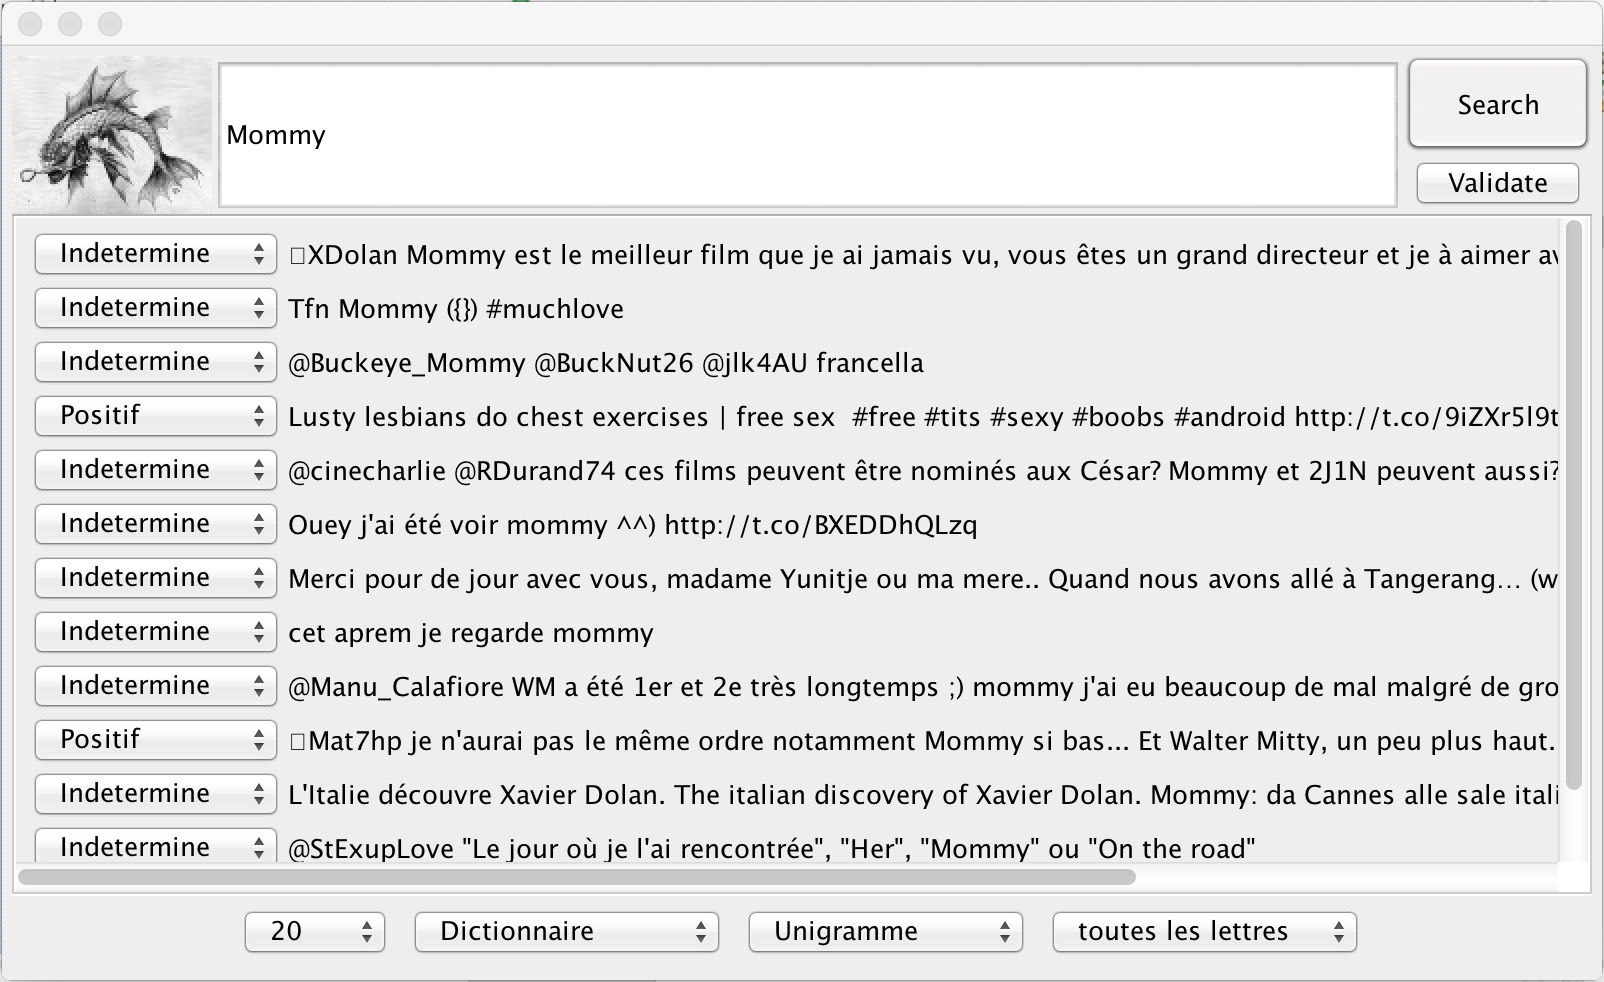
\includegraphics[scale=0.26]{img/BehAnTweet_Dict_20.jpeg}

Visualisation des tweets recueillis avec le mot-clef "Mommy", et la méthode de classification "Dictionnaire".
\\
La classification se trouvant à gauche de chaque contenu de tweet pourra être modifiable - on pourra alors choisir pour chaque tweet d'une classification "Positif", "Négatif" et "Indéterminé". Une fois la modification effectuée (ou non), on pourra valider la classification de tous les tweets en cliquant sur le bouton "Validate", qui enregistrera dans la base d'apprentissage la liste des tweets classifiés.
\\

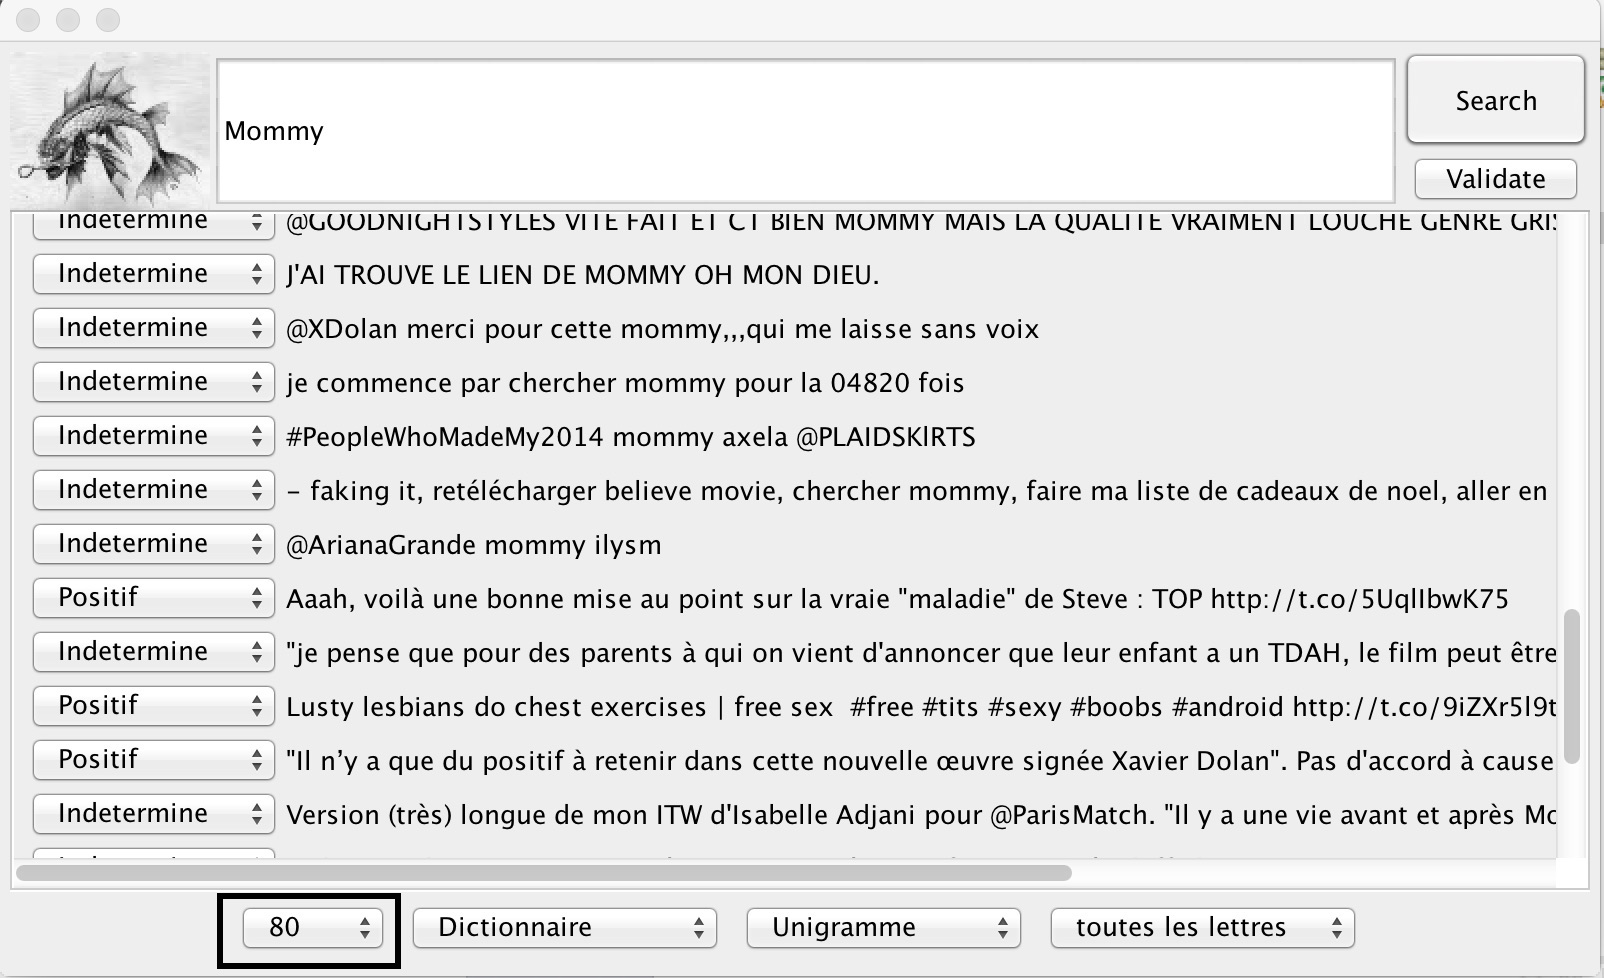
\includegraphics[scale=0.52]{img/BehAnTweet_Dict_80_annotation.jpeg}

Modification du nombre de tweets à recueillir - au maximum 80.

\subsection{Manuel d'utilisation}

\subsubsection{Comment modifier les paramètres réseaux de l'application?}

Ouvrez le fichier \textit{twitter4j.properties}.
\\
Recherchez les deux lignes situées sous le commentaire : //PROXY.
\\
\\
\underline{Si vous vous trouvez sur l'Université Lille1}, veuillez entrer les propriétés proxy : 
\\	http.proxyHost=cache-etu.univ-lille1.fr
\\	http.proxyPort=3128
\\
\\
\underline{Si vous ne vous trouvez pas sur sur l'Université Lille1}, vous pouvez désactiver les propriétés proxy en commentant les lignes précédentes.

\subsubsection{Comment modifier le nombre de tweets recueillis pour une requête?}

Dans l'encart des paramètres, cliquez sur le bouton "20" - cela signifie que le nombre de tweets maximal affiché est de 20.
\\
Cliquez alors sur la nouvelle valeur que vous voulez prendre en compte.

\subsubsection{Comment modifier la méthode de classification pour une requête?}

Dans l'encart des paramètres, cliquez sur le bouton "Dictionnaire", et choisissez alors votre méthode de classification.
\\
Si vous choisissez la méthode Bayes Fréquence, choisissez alors le nombre de grammes que vous voulez utiliser, et enfin le "type" de mots que vous voulez comparer - avec le nombre de lettres par mot.

\subsubsection{Comment effectuer une requête?}

Vous pouvez effectuer une recherche en tapant votre requête dans la barre de recherche de tweet. Après cela, vous pouvoir choisir dans l'encart de paramètres le nombre de tweets maximal à recueillir pour cette requête, ainsi que la méthode de classification demandée.
\\
Après le choix des paramètres, cliquez sur le bouton "Search" afin de lancer votre requête, via \textit{Twitter4J} et l'API Twitter. Vous obtiendrez alors dans l'encart de visualisation, quelques secondes après, un ensemble de tweets recueillis et en lien à cette recherche.

\subsubsection{Comment modifier la classification d'un ou de plusieurs résultat(s) de requêtes?}

Après une requête, vous pouvez remarquer dans l'encart de visualisation que, via la méthode de classification choisie, une classification est déjà établie - à gauche du tweet.
\\
Si la classification d'un tweet ne vous plaît pas, vous pouvez la modifier en cliquant sur la classification du tweet. Vous pouvez alors choisir la classification qui vous plaît, en cliquant sur celle choisie.
\\
Vous pourrez alors constater que votre demande a bien été prise en compte, via le changement de la classification dans l'encart de visualisation.

\subsubsection{Comment enregistrer les résultats d'une requête dans la base d'apprentissage?}

Une fois les classifications de chaque tweet analysées, vous pouvez enregistrer celles-ci dans la base d'apprentissage, en vue d'une nouvelle recherche avec une méthode de classification KNN ou de Bayes.
\\
Pour cela, il vous suffit juste de cliquer sur le bouton "Validate", présent dans l'encart de recherche. Une fois cliqué, le bouton devient gris - il ne vous ai plus possible de valider une seconde fois ces mêmes classifications.

\chapter{Algorithmes de classification}

Pour l'analyse de tweets, divers algorithmes de classification ont été utilisés.\\
Voici la liste des algorithmes de classification utilisés.

\section{Dictionnaire}

L'algorithme \textbf{Dictionnaire} est l'algorithme le plus facile à programmer.\\
En effet, il consiste dans un premier temps à obtenir une liste de mots positifs et négatifs. Chaque tweet sera découpé en mots, et chaque mot sera confondu avec les deux listes - aussi, le tweet partira avec un score entier nul. Si un des mots du tweet est reconnu dans la liste de mots positifs, on diminuera son score - à contrario, si ce mot est reconnu dans la liste de mots négatifs, on augmentera son score.\\
Finalement, on obtiendra pour un tweet un score, somme des scores de chaque mot appartenant à celui-ci. Ce score décidera de la classification auquel appartient le tweet:
\begin{itemize}
\item{positif, si le score est négatif,}
\item{indéterminé, si le score est nul,}
\item{négatif, si le score est positif.}
\end{itemize}
La critique première qui peut être faite pour cette méthode de classification est qu'il est nécessaire de donner tous les mots possibles pour classifier un tweet - aussi, cette méthode ne gère pas le cynisme, ironie et sarcasme des tweets, car cet algorithme ne travaille pas sur une base d'apprentissage.

\section{KNN}

La méthode KNN, ou des \textit{k} plus proches voisins, est une méthode d'apprentissage automatique basée sur des exemples contenus dans une base d'apprentissage.
On cherchera ici à trouver les \textit{k} plus proches tweets du tweet analysé, contenus dans la base d'apprentissage du projet\footnote{Cette base d'apprentissage consiste en la sauvegarde de tweets déjà analysés pour le comportement.}.
\\
Pour chaque tweet, on aura un tableau de \textit{k} objets, contenant un couple (distance, tweet). On range ainsi les \textit{k} premiers tweets de la base d'apprentissage dans le tableau énoncé précédemment, les distances étant calculées entre le tweet à classifier et le tweet de la base d'apprentissage selon la formule suivante : \textbf{((nombreMotsTotal) - nombreMotsCommuns) / nombreMotsTotal}.
Pour les (\textit{k}+1) à \textit{n}\footnote{\textit{n} étant le nombre de tweets total contenus dans la base d'apprentissage.} tweets, on calculera à chaque fois la distance entre le tweet courant et le tweet à classifier. Si cette distance est inférieure à la plus grande distance contenue dans le tableau des \textit{k} objets, on remplacera alors cet objet par la nouvelle distance ainsi que le tweet courant associé à celle-ci.
\\
Une fois cette étape faite, il nous restera à définir le comportement du tweet à classifier - pour cela, on comptera combien il y a de tweets positifs issus de la base d'apprentissage, de même pour les tweets négatifs et indéterminés. Le score le plus élevé parmi les 3 sera l'avis décisif pour le tweet à classifier.

\section{Bayes}

La classification Bayésienne est, quant à elle, basée sur les probabilités conditionnelle et la règle de Bayes. Aussi, on se servira d'une base d'apprentissage, car nous avons besoin de connaissances afin de pouvoir classifier les tweets recueillis.\\
Pour la méthode Bayes, nous utiliserons deux sous-méthodes de classification: \textit{Présence} et \textit{Fréquence}. Pour la classification par Fréquence, on estimera la probabilité d'occurence d'un événement, ce qui n'est pas pris en compte pour la classification par Présence.

\subsection{Présence}

On devra déterminer la classe la plus probable pour un tweet. Pour cela, on utilisera la règle de Bayes : P(\textit{c} | \textit{t}) = P(\textit{t} | \textit{c}) . P(\textit{c}) / P(\textit{t}), où \textit{c} est la classe d'un tweet (Positif, Négatif ou Indétermine), et \textit{t} le tweet à classifier.
\\
Dans cette sous-méthode, on ne se préoccupe pas du nombre d'occurrences des mots.

\subsection{Fréquence}

Dans cette sous-méthode, on prendra en compte le nombre d'occurrences d'un mot du tweet à classifié.
\\
On pourra considérer ici plusieurs combinaisons de mots:
\begin{itemize}
\item{uni-gramme}
\item{bi-gramme : chef d'oeuvre}
\end{itemize}
Aussi, on pourra considérer de calculer cette fréquence sur tous les mots du tweet, ou alors sur seulement des mots ayant un certain nombre de lettres pour ne pas être considérés comme des mots inutiles (comme "le", "la", "les", "de", "du", ...).
\\
Tout ceci pourra réduire les calculs (sans affecter le modèle de classifier), et marquer l'importance de certains mots ou certains groupes de mots. 

\chapter{Résultats de la classification}

\section{Dictionnaire}

Cet algorithme, facile à implémenter, est malheureusement peu fiable mais aussi assez lent. En effet, il s'appuie sur deux dictionnaires : un dictionnaire positif et un négatif. Comme dit précédemment, l'algorithme ne gère pas le cynisme, ironie et sarcasme des tweets. Mais surtout, il ne comptabilise pas les mots qui ne sont pas présents dans les deux dictionnaires, ce qui est n'est pas évident pour la conjugaison d'un verbe par exemple, ou alors lors d'une malencontreuse faute d'orthographe dans le mot.
\\
Aussi, l'algorithme est lent car, à chaque tweet, il doit regarder si chaque mot issu du dictionnaire positif est présent dans le tweet à analyser - de même pour le dictionnaire négatif.

\chapter{Conclusion}

\chapter*{Bibliographie - Webographie}

\end{spacing}
\end{document}